\documentclass[../main.tex]{subfiles}
\graphicspath{{\subfix{../images/}}}
\begin{document}
\section*{Term 1 Week 6}
\begin{enumerate}
    \item 
    Solve for \(x\):\\
    \begin{figure}[h]
        \centering
        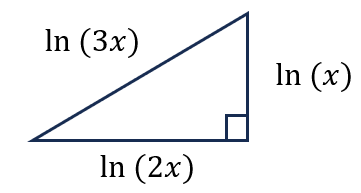
\includegraphics{images/t1w6q1.png}
    \end{figure}\\

    \item 
    Solve for \(x\):\\

    \setlength{\parindent}{30pt}
    \(\log_5(x)+\log_7(x)=\log_{25}(x)\)\\

    \item 
    Show that the equation \(4x^2-y^2-16hx+2hy+15h^2-4a^2=0\), where \textit{h} and \textit{a} are positive constants, represents a hyperbola.\\
    
    \setlength{\parindent}{0pt}
    If the tangent to this hyperbola at the point \((p,q)\) is parallel to the straight line \(y=(e^2-1)x\), where \textit{e} is the eccentricity of the hyperbola, show that \(p-q=h \).\\

    Note: the eccentricity of the hyperbola \(\frac{x^2}{a^2}-\frac{y^2}{b^2}=1\) is given by \(e^2=1+\frac{b^2}{a^2}\)
    
\end{enumerate}

\end{document}